\documentclass[usenames,svgnames,14pt]{beamer}
\usepackage[english]{babel}
\usepackage{
  fontspec,
  fontawesome,
  xcolor,
  mathabx,
  listings,
  lstautogobble,
  listofitems,
  TeXnicalities,
  array,
  pgfplotstable,
  pifont
}
\pgfplotsset{compat=1.17}

\setsansfont{Yanone Kaffeesatz}[
    UprightFont     = *-Regular ,
    BoldFont        = *-Bold ,
    BoldItalicFont  = *-Bold ,
    BoldSlantedFont = *-Bold ,
    ItalicFont      = *-Light ,
    SlantedFont     = *-Light ,
    SmallCapsFont   = *-Thin
]
\graphicspath{{../Figures/},{../Figures/Gitflow},{../Figures/Meme}}
\usetheme[style=green]{Z02}

\usetikzlibrary{
    positioning,
    shapes,
    bbox
}
%Colors for listings
\colorlet{background-color}{gray!20}
\colorlet{basic-color}{black}
\colorlet{keywords-color}{Goldenrod}
\colorlet{comment-color}{red!95!black}
\colorlet{strings-color}{ForestGreen}
\colorlet{builtins-color}{MediumBlue!90!black}
\colorlet{functions-color}{NavyBlue}
\colorlet{variables-color}{DarkOrange}
\colorlet{environment-color}{Gray}
\colorlet{external-color}{SteelBlue}

% https://tex.stackexchange.com/a/34000
\makeatletter
\lst@Key{countblanklines}{true}[t]%
    {\lstKV@SetIf{#1}\lst@ifcountblanklines}

\lst@AddToHook{OnEmptyLine}{%
    \lst@ifnumberblanklines\else%
       \lst@ifcountblanklines\else%
         \advance\c@lstnumber-\@ne\relax%
       \fi%
    \fi}
\makeatother

%listings set
\lstdefinestyle{MyBash}{
backgroundcolor=\color{background-color}, % choose the background color; you must add \usepackage{color} or \usepackage{xcolor}
breakatwhitespace=false,            % sets if automatic breaks should only happen at whitespace
breaklines=true,                    % sets automatic line breaking
captionpos=b,                       % sets the caption-position to bottom
deletekeywords={...},               % if you want to delete keywords from the given language
escapeinside={@|}{|@},              % if you want to add LaTeX within your code
extendedchars=true,                 % lets you use non-ASCII characters; for 8-bits encodings only,
                                    % does not work with UTF-8
frame=single,                       % adds a frame around the code
framerule=0pt,                      % Width of the frame rule
framesep=3pt,                       % separation around text
linewidth=\textwidth,               % defines the base line width for listings
xleftmargin=6mm,                    % Margin left
xrightmargin=6mm,                   % Margin right
numbers=left,                       % where to put the line-numbers; possible values are (none, left, right)
numberblanklines=false,             % suppress numbers on empty lines
countblanklines=false,              % NOT standard! Avoid counting empty lines: https://tex.stackexchange.com/a/34000
numbersep=8pt,                      % how far the line-numbers are from the code
numberstyle=\tiny\color{black},     % the style that is used for the line-numbers
rulecolor=\color{black},            % if not set, the frame-color may be changed on line-breaks within not-black text
                                    % (e.g. comments (green here))
showspaces=false,                   % show spaces everywhere adding particular underscores; it overrides 'showstringspaces'
showstringspaces=false,             % underline spaces within strings only
showtabs=false,                     % show tabs within strings adding particular underscores
stepnumber=1,                       % the step between two line-numbers. If it's 1, each line will be numbered
tabsize=2,                          % sets default tabsize to 2 spaces
title=\lstname,                     % show the filename of files included with \lstinputlisting; also try caption instead of title
%
%Base style for this presentation 
keepspaces=true,                    % keeps spaces in text, useful for keeping indentation of code
                                    % (possibly needs columns=flexible)
language=bash,
basicstyle=\ttfamily\scriptsize\color{basic-color},
keywordstyle=\color{keywords-color},
stringstyle=\color{strings-color},
commentstyle=\color{comment-color},
morestring=[b][\color{strings-color}]{"},
morestring=[d][\color{strings-color}]{'},
moredelim=[is][\color{basic-color}]{|+}{+|}, % I will use this for terminal output
literate={`}{\textasciigrave}1, % https://tex.stackexchange.com/a/466224/128737
literate={~}{{\textasciitilde}}1,
% literate=% literate={<replace>}{<replacement text>}{<width>}
%   {\#define}{{{\color{CarnationPink}\#define}}}{6}
%   {\#include}{{{\color{CarnationPink}\#include}}}{7},
alsoletter=0123456789![]/\{\}.:+, % This to mark the symbols in keyword/emph[5] to be highlighted (otherkeywords does not work i.e. it highlights also in comments!) -> manual at page 45
morekeywords={if, then, else, elif, fi, case, esac, for, select, while, until, do, done, in, function, time, [[, ]], \{, \}, !, coproc}, %https://askubuntu.com/a/513712
emph=[1]{},
emphstyle=[1]{\color{functions-color}}, %Functions
emph=[2]{},
emphstyle=[2]{\color{variables-color}}, %Variables
emph=[4]{PATH, SHELL, IFS, BASH_ALIASES, BASH_REMATCH, PS3, REPLY, HOME, LANGUAGE, EDITOR, PIPESTATUS, PWD, FUNCNEST,
         DIRSTACK, PWD, OLDPWD, SHELLOPTS, BASHOPTS, TIMEFORMAT, COMP_CWORD, COMP_LINE, COMP_POINT, COMP_TYPE, COMP_KEY,
         COMP_WORDBREAKS, COMP_WORDS, COMPREPLY, INPUTRC},
emphstyle=[4]{\color{environment-color}}, %Environment variables
emph=[5]{alias, bg, bind, break, builtin, cd, command, compgen, complete, continue, declare, dirs, disown, echo, enable, eval,
         exec, exit, export, false, fc, fg, getopts, hash, help, history, jobs, kill, let, local, logout, popd, printf, pushd, pwd,
         read, readonly, return, set, shift, shopt, source, suspend, test, times, trap, true, type, typeset, ulimit, umask,
         % case, if, until, while  % <--- these built-in are keywords and I leave them highlighted as such
         unalias, unset, wait, :, ., [, ]},
emphstyle=[5]{\color{builtins-color}}, %Shell built-in
emph=[6]{man, apropos, ls, rm, g++, chmod, cp, awk, sed, cut, perl, args, date, grep, sleep, tput, seq, cat, wc, sort, uniq, tail,
         head, sdiff, tar, mktemp, mkdir, ps, emacs, systemd, timeout, parallel, xargs, gnuplot, pdflatex, vi, ping, bash,
         egrep, shuf, stat, find, fgrep, bc, tr, paste, expr, diff, touch},
emphstyle=[6]{\color{external-color}}, %(External) commands
emph=[7]{},
emphstyle=[7]{\color{variables-color}}, %Class for local variables (usually with bad names)
emph=[8]{},
emphstyle=[8]{\color{builtins-color}}, %Class for local commands (usually with bad names)
%
%Additional customizations
belowskip=-7mm,
aboveskip=3pt,
autogobble=true, % lstautogobble needed!
}

\lstnewenvironment{Bash}[1][] %I will rarely use this because putting a $ in it as prompt breaks down TeXclipse highlight syntax!
    {\lstset{style=MyBash, #1}}
    {}

\def\bash{\lstinline[style=MyBash, basicstyle=\ttfamily\color{black}]}

%\includeonlyframes{current}

%This command set the \HeightOfNode \WidthOfNode pgfmath macro
\newcommand{\CalculateSizeOfNode}[1]{%
    \pgfpointdiff{\pgfpointanchor{#1}{south west}}{\pgfpointanchor{#1}{north east}}
    \pgfmathsetmacro\WidthOfNode{\csname pgf@x\endcsname}
    \pgfmathsetmacro\HeightOfNode{\csname pgf@y\endcsname}
}

%Inspired from https://tex.stackexchange.com/a/87518/128737
%To be called in tikzpicture!
% #1 -> width rectangle where to place
% #2 -> height rectangle where to place
% #3 -> radius of empty space around coordinate (without units, in pt)
% #4 -> how many coordinate to place
%
% It defines tikz coordinates called 'N1', 'N2', etc. in a rectangle (0,0) to (#3, #4)
\newcommand{\PlaceSpreadCoordinatesAndStoreThemToFile}[4]{
    \newwrite\posfile
    \immediate\openout\posfile=\jobname .pos
    \def\xlist{6}
    \def\ylist{6}
    \newcounter{NodeIndex}
    \pgfmathtruncatemacro\Width{0.0351459804*#1}
    \pgfmathtruncatemacro\Height{0.0351459804*#2}
    \pgfmathsetmacro\diameter{#3}
    \draw (0,0) rectangle (\Width,\Height);
    \foreach \i in {1,...,#4}{
        \xdef\collision{1}
        \whileboolexpr{test {\ifnumcomp{\collision}{=}{1}}}{%
            \pgfmathsetmacro\x{rnd*\Width}
            \pgfmathsetmacro\y{rnd*\Height}
            \xdef\collision{0}
            \foreach \element [count=\i] in \xlist{
                \pgfmathtruncatemacro\j{\i-1}
                \pgfmathsetmacro\checkdistance{ sqrt( ({\xlist}[\j]-(\x))^2 + ({\ylist}[\j]-(\y))^2 ) }
                \ifdim\checkdistance pt<\diameter pt
                \xdef\collision{1}
                \breakforeach
                \fi
            }
        }
        \ifnum\collision=0
        \xdef\xlist{\xlist,\x}
        \xdef\ylist{\ylist,\y}
        \stepcounter{NodeIndex}
        \coordinate (C\theNodeIndex) at (\x,\y);
        \node at (C\theNodeIndex) {\immediate\write\posfile{\x\space \y}};
        \message{Placed node \theNodeIndex^^J}
        \fi
    }
}

% Branch for gitflow
\newcommand{\mainBranchColor}{PQ}
\newcommand{\supportBranchColor}{Marine}
\newcommand{\branch}[2]{\textcolor{#1}{\texttt{\bfseries #2}}}
\newcommand{\main}{\branch{\mainBranchColor}{main}}
\newcommand{\develop}{\branch{\mainBranchColor}{develop}}
\newcommand{\feature}{\branch{\supportBranchColor}{feature}}
\newcommand{\release}{\branch{\supportBranchColor}{release-*}}
\newcommand{\hotfix}{\branch{\supportBranchColor}{hotfix-*}}

% Further utilities
\renewcommand{\checkmark}[1][PP]{\textcolor{#1}{\ding{51}}}
\newcommand{\crossmark}[1][PT]{\textcolor{#1}{\ding{55}}}

%===============================================================%
\title{Git in real life}
\date{16 December 2022}
\author{Alessandro Sciarra}
\institute{Z02~--~Software Development Center}
\titlegraphic{
\includegraphics[width=20mm]{LogoCRC}}
\titlepagelogo{
\includegraphics[width=20mm]{LogoGoethe}}
%===============================================================%

\AtBeginSection[] % <- Empty optional argument, do nothing for \section*
{
    \begin{frame}[plain, noframenumbering]{}
         \sectionpage
    \end{frame}
}

\tikzset{
    space/.style={%
        thick, draw=#1, fill=#1!10, text=#1, rounded corners=1mm, font=\small, text width=14mm, align=center, minimum height=12mm
    },
    commit/.style={circle, draw, very thick, fill=#1, minimum size=5mm},
    branch/.style={rounded corners=1mm, fill=#1, draw, very thick, font=\small},
    pin/.style={to, thick, shorter={1pt}{1pt}}
}
\newcommand{\labelBranch}[5]{%
    \node[#2 = #3 of #4, branch=#5] (tmp) {#1\vphantom{FMi}};
    % https://tex.stackexchange.com/a/24924
    \expandafter\ifstrequal\expandafter{#2}{above}{\draw[pin] (tmp.south) -- (#4.north);}{}
    \expandafter\ifstrequal\expandafter{#2}{below}{\draw[pin] (tmp.north) -- (#4.south);}{}
    \expandafter\ifstrequal\expandafter{#2}{right}{\draw[pin]  (tmp.west) -- (#4.east);}{}
    \expandafter\ifstrequal\expandafter{#2}{left}{ \draw[pin]  (tmp.east) -- (#4.west);}{}
}
\PrepareURLsymbol[PB]
\newcommand{\ttc}[2]{\texttt{\textcolor{#1}{#2}}}%
\setlength{\leftmarginii}{0.5cm}
\newcommand{\then}{\raisebox{2pt}{$\;\drsh\;$}}


% Taken from https://tex.stackexchange.com/a/51458/128737
\makeatletter
\patchcmd{\beamer@sectionintoc}{\vskip1.5em}{\vskip0.5em}{}{}
\makeatother

\begin{document}

%===============================================================%
\begin{frame}[plain,noframenumbering]
    \titlepage
    \begin{tikzpicture}[remember picture, overlay]
        \node[anchor=south, font=\small, text=BGLIGHT]
            at ($(current page.center)!0.95!(current page.south)$)
            {\href{https://github.com/AxelKrypton}{\faGithub\,AxelKrypton}};
    \end{tikzpicture}
\end{frame}
%~~~~~~~~~~~~~~~~~~~~~~~~~~~~~~~~~~~~~~~~~~~~%
\begin{frame}{Outline of the talk}
    \tableofcontents[subsectionstyle=hide]
\end{frame}
%===============================================================%


%===============================================================%
\section{Rewriting history}
%~~~~~~~~~~~~~~~~~~~~~~~~~~~~~~~~~~~~~~~~~~~~%
\begin{frame}{About rewriting history}{Yes, you can change the history of a repository!}
\begin{overlayarea}{\textwidth}{0.3\textheight}
    \setlength{\leftmargini}{5mm}
    \begin{itemize}
        \item\alert{Very bad if there are different copies of the history} \Remark{E.g.\ branches, remote(s)}
        \item If you rewrite shared history,\\
              \begin{itemize}
                  \item it is generally hard to make the same change elsewhere and\\
                  \item merging (and hence pull/push) can lead to duplicated commits in history
              \end{itemize}
        \item<only@1> Fine as long as\\
              \begin{itemize}
                  \item yours is the only clone containing the rewritten history or
                  \item you work on a git project alone and you know what to do then
              \end{itemize}
    \end{itemize}
\end{overlayarea}
    \begin{center}
        \begin{tikzpicture}[scope on=<2->]
            \draw[very thick] (-0.5,2) -- (4,2);
            \draw[very thick] (-0.5,0) -- (4,0);
            \draw[dashed] (4,2) -- node[pos=0.35, font=\scriptsize, fill=BGLIGHT, inner ysep=2pt] {Up-to-date} (4,0);
            \foreach \x [count=\i from 1] in {0,1,...,4}{
                \node[commit=PP!70] (R\i) at (\x,2) {};
            }
            % Branch labels
            \node[right = of R5, branch=PP!80] (BrR) {Remote main};
            % Complete paths
            \draw[pin] (BrR.west) -- (R5.east);
            \begin{scope}[scope on=<2>]
                \foreach \x [count=\i from 1] in {0,1,...,4}{
                    \node[commit=PS!70] (L\i) at (\x,0) {};
                }
                % Branch labels
                \node[right = of L5, branch=PS!50] (BrL) {Local main};
                % Complete paths
                \draw[pin] (BrL.west) -- (L5.east);
            \end{scope}
            \begin{scope}[scope on=<3>]
                \node (cross) at (4,0.7) {};
                \fill[BGLIGHT] ($(cross.south west)-(0,1)$) rectangle (cross.north east);
                \draw[ultra thick, red] (cross.south west) -- (cross.north east) (cross.south east) -- (cross.north west);
                \foreach \x [count=\i from 1] in {0,1,...,4}{
                    \ifnum\x>1
                        \node[commit=PT!70] (L\i) at (\x,0) {};
                    \else
                        \node[commit=PS!70] (L\i) at (\x,0) {};
                    \fi
                }
                % Branch labels
                \node[right = of L5, branch=PS!50] (BrL) {Local main};
                \node at (BrR) {\includegraphics[width=18mm]{boom}};
                % Complete paths
                \draw[pin] (BrL.west) -- (L5.east);
            \end{scope}
        \end{tikzpicture}
        \par\uncover<3>{\small\alert{As soon as you rewrite history contained elsewhere, you are in troubles!}}
    \end{center}
    \begin{tikzpicture}[remember picture, overlay]
        \node[anchor=north east] at ([xshift=-12mm]current page.north east) {
\includegraphics[width=25mm]{Spiderman}};
    \end{tikzpicture}
\end{frame}
%~~~~~~~~~~~~~~~~~~~~~~~~~~~~~~~~~~~~~~~~~~~~%
\begin{frame}[fragile]{Changing the last commit (message)}
    \begin{enumerate}
        \item How can I fix a typo in the \textbf{last} commit message?
    \end{enumerate}
    \begin{varblock}{alerted}[\textwidth]{This procedure will change history!}
        Said differently, feel free to do it if you \alert{\textbf{did not}} share history!
    \end{varblock}
    \vspace{3mm}
    \begin{onlyenv}<1>
        \begin{lstlisting}[style=MyBash]
            $ git commit -m "Added engine implementation"
            |+[airplane f8b0c25] Added engine implementation
            24 files changed, 1340 insertions(+), 476 deletions(-)+|
            # Ops! I used a verb in past form, @|\URL[red]{https://chris.beams.io/posts/git-commit/}{not conforming!}|@
        \end{lstlisting}
    \end{onlyenv}
    \begin{onlyenv}<2>
        \begin{lstlisting}[style=MyBash]
            $ git commit -m "Added engine implementation"
            |+[airplane +||*f8b0c25*||+] Added engine implementation
            24 files changed, 1340 insertions(+), 476 deletions(-)+|
            # Ops! I used a verb in past form, @|\URL[red]{https://chris.beams.io/posts/git-commit/}{not conforming!}|@
        \end{lstlisting}
    \end{onlyenv}
    \begin{uncoverenv}<2>
        \begin{lstlisting}[style=MyBash]
            # With clean staging area:
            $ git commit --amend -m "Add engine implementation"
            |+[airplane +||*33f53f4*||+] Add engine implementation
            Date: Fri Nov 25 08:02:22 2022 +0100
            24 files changed, 1340 insertions(+), 476 deletions(-)+|
        \end{lstlisting}
    \end{uncoverenv}
    \FrameRemark{There is a \URL*{https://git-scm.com/book/en/v2/Git-Tools-Rewriting-History}{nice official page} about different situations in which rewriting history is needed.}
\end{frame}
%~~~~~~~~~~~~~~~~~~~~~~~~~~~~~~~~~~~~~~~~~~~~%
\begin{frame}[fragile]{Changing the last commit (content)}
    \begin{enumerate}
        \setcounter{enumi}{1}
        \item I forgot some changes in the \textbf{last} commit! And now?
    \end{enumerate}
    \begin{varblock}{alerted}[\textwidth]{This procedure will change history!}
        Said differently, feel free to do it if you \alert{\textbf{did not}} share history!
    \end{varblock}
    \vspace{3mm}
    \begin{onlyenv}<1>
        \begin{lstlisting}[style=MyBash]
            $ git commit -m "Review take-off system"
            |+[airplane e1df32a] Review take-off system
            1 file changed, 230 insertions(+), 61 deletions(-)+|
            # Ops! I forgot a file!
        \end{lstlisting}
    \end{onlyenv}
    \begin{onlyenv}<2-3>
        \begin{lstlisting}[style=MyBash]
            $ git commit -m "Review take-off system"
            |+[airplane +||*e1df32a*||+] Review take-off system
            1 file changed, 230 insertions(+), 61 deletions(-)+|
            # Ops! I forgot a file!
        \end{lstlisting}
    \end{onlyenv}
    \begin{onlyenv}<1-2>
        \begin{uncoverenv}<2>
            \begin{lstlisting}[style=MyBash]
                $ git add wheels_electronic.h
                $ git commit --amend --no-edit
                |+[airplane +||*c13e34f*||+] Add engine implementation
                Date: Fri Nov 25 08:45:18 2022 +0100
                2 files changed, 345 insertions(+), 88 deletions(-)+|
            \end{lstlisting}
        \end{uncoverenv}
    \end{onlyenv}
    \begin{onlyenv}<3>
    \begin{lstlisting}[style=MyBash]
            $ git add wheels_electronic.h
            $ git commit --amend -C HEAD # use original commit timestamp
            |+[airplane +||*c13e34f*||+] Add engine implementation
            Date: Fri Nov 25 08:33:01 2022 +0100
            2 files changed, 345 insertions(+), 88 deletions(-)+|
        \end{lstlisting}
    \end{onlyenv}
    \FrameRemark{There is a \URL*{https://git-scm.com/book/en/v2/Git-Tools-Rewriting-History}{nice official page} about different situations in which rewriting history is needed.}
\end{frame}
%===============================================================%


%===============================================================%
\section{Git rebase}
%~~~~~~~~~~~~~~~~~~~~~~~~~~~~~~~~~~~~~~~~~~~~%
\begin{frame}{Which is the abstract idea of a rebase?}
    \vspace{-3mm}
    \begin{enumerate}
        \item<2-> Go back in history till a \textbf{given} point
        \item<3-4> Replay \textbf{chosen} commits in their order\\
                   \then possibly taking action on applied commit as specified
    \end{enumerate}
    \vspace{3mm}
    \begin{tikzpicture}
        \draw[very thick] (-0.5,1.2) -- (6,1.2);
        \foreach \x [count=\i from 1] in {0,1.5,...,6.1}{
            \node[commit=PS!70] (I\i) at (\x,1.2) {};
        }
        \node[above = 6mm of I5, branch=PS!80] (BrI) {main};
        \draw[pin] (BrI.south) -- (I5.north);
        \node[above = 6mm of I2, font=\small\ttfamily] {Before rebase};
        \draw[thin] (-2,0.6) -- (8,0.6);
        \begin{scope}[scope on=<2->]
           \draw[very thick] (-0.5,0) -- (3,0);
            \foreach \x [count=\i from 1] in {0,1.5,3}{
                \node[commit=PS!70] (R\i) at (\x,0) {};
            }
        \end{scope}
        \begin{onlyenv}<2> % Use onlyenv because of opacities
            \begin{scope}
                \draw[very thick, opacity=0.2] (3.25,0) -- ++(1,0) (4.75,0) -- ++(1,0);
                \foreach \x [count=\i from 4] in {4.5,6.0}{
                    \node[opacity=0.2, commit=PS!70] (R\i) at (\x,0) {};
                }
                % Branch label
                \node[below = 6mm of R3, branch=PS!80] (BrR) {main};
                % Complete paths
                \draw[pin] (BrR.north) -- (R3.south);
                \node[below = 6mm of R5, font=\small\ttfamily] {During rebase};
            \end{scope}
        \end{onlyenv}
        \begin{onlyenv}<3>
            \begin{scope}
                \draw[very thick] (3.25,0) -- (4.5,0);
                \draw[very thick, opacity=0.2] (4.75,0) -- ++(1,0);
                \node[commit=PT!70] (R4) at (4.5,0) {};
                \node[opacity=0.2, commit=PS!70] (R5) at (6,0) {};
                % Branch label
                \node[below = 6mm of R4, branch=PS!80] (BrR) {main};
                % Complete paths
                \draw[pin] (BrR.north) -- (R4.south);
                \node[below = 6mm of R2, font=\small\ttfamily] {During rebase};
            \end{scope}
        \end{onlyenv}
        \begin{scope}[scope on=<4>]
            \draw[very thick] (3.25,0) -- (6,0);
            \node[commit=PT!70] (R4) at (4.5,0) {};
            \node[commit=PT!70] (R5) at (6,0) {};
            % Branch label
            \node[below = 6mm of R5, branch=PS!80] (BrR) {main};
            % Complete paths
            \draw[pin] (BrR.north) -- (R5.south);
            \node[below = 6mm of R2, font=\small\ttfamily] {After rebase};
        \end{scope}
    \end{tikzpicture}
\end{frame}
%~~~~~~~~~~~~~~~~~~~~~~~~~~~~~~~~~~~~~~~~~~~~%
\begin{frame}{Rebasing instead of (three-way) merging}
    \vspace{1mm}
    Three way merge from Feature:
    \begin{center}
        \begin{tikzpicture}
            \draw[very thick] (0.5,0) -- (2.5,0) edge[out=0, in=180] (3.5,1) (3.5,1) -- (5,1);
            \draw[very thick] (2.5,0) -- (5.5,0);
            \foreach \dx/\dy [count=\i from 1] in {1/0, 2/0, 3.3/0, 4.5/0, 5.7/0, 4/1, 5/1}{
                \ifnum\i<6
                   \def\col{PS!50}
                \else
                    \def\col{white}
                \fi
                \node[commit=\col] (C\i) at ($(0,0)+(\dx,\dy)$) {};
            }
            \labelBranch{main}{below}{5mm}{C5}{PS!50}
            \begin{scope}[scope on=<1>]
                \labelBranch{Feature}{right}{5mm}{C7}{white}
            \end{scope}
            \begin{scope}[scope on=<2->]
                \draw[very thick] (5.25,1) -- (7.7,1);
                \draw[very thick] (5.95,0) -- (6.2,0)  edge[out=0, in=180] (7.2,1);
                \node[commit=white] (CM) at (7.7,1) {};
                \node[font=\tiny] at (CM) {$\star$};
                \labelBranch{Feature}{right}{5mm}{CM}{white}
                \node[below = 16mm of CM, anchor=west, font=\scriptsize] {$^\star$Conflicts might occur};
            \end{scope}
        \end{tikzpicture}
    \end{center}
    \vspace{-2mm}
    Rebase from Feature:
    \par\vspace{-1mm}
    \begin{center}
        \begin{tikzpicture}
            \draw[very thick] (0.5,0) -- (5.5,0);
            \foreach \dx/\dy [count=\i from 1] in {1/0, 2/0, 3.3/0, 4.5/0, 5.7/0}{
                \node[commit=PS!50] (C\i) at ($(0,0)+(\dx,\dy)$) {};
            }
            \labelBranch{main}{below}{5mm}{C5}{PS!50}
            \begin{scope}[scope on=<1-2>]
                \draw[very thick] (2.5,0) edge[out=0, in=180] (3.5,1) (3.5,1) -- (5,1);
                \foreach \dx/\dy [count=\i from 6] in {3.9/1, 5.1/1}{
                    \node[commit=white] (C\i) at ($(0,0)+(\dx,\dy)$) {};
                }
                \labelBranch{Feature}{right}{5mm}{C7}{white}
            \end{scope}
            \begin{onlyenv}<3> % Because of opacity
                \begin{scope}
                    \draw[opacity=0.2, very thick] (2.5,0) edge[out=0, in=180] (3.5,1)
                                                   (3.5,1) -- ++(0.15,0) +(0.5,0) -- ++(1.2,0);
                    \foreach \dx/\dy [count=\i from 6] in {3.9/1, 5.1/1}{
                        \node[opacity=0.2, commit=white] (C\i) at ($(0,0)+(\dx,\dy)$) {};
                    }
                    \labelBranch{Feature}{right}{5mm}{C5}{white}
                \end{scope}
            \end{onlyenv}
            \begin{scope}[scope on=<4->]
                \draw[very thick] (5.95,0) -- (6.2,0) edge[out=0, in=180] (7.2,1) (7.2,1) -- ++(0.15,0);
                \node[commit=white] (C6) at (7.6,1) {};
                \node[font=\tiny] at (C6) {$\star$};
            \end{scope}
            \begin{onlyenv}<4> % Because of opacity
                \begin{scope}
                    \draw[opacity=0.03, very thick] (2.5,0) edge[out=0, in=180] (3.5,1)
                        (3.5,1) -- ++(0.15,0) +(0.5,0) -- ++(1.2,0);
                    \foreach \dx/\dy [count=\i from 6] in {3.9/1, 5.1/1}{
                        \node[opacity=0.03, commit=white] at ($(0,0)+(\dx,\dy)$) {};
                    }
                    \draw[opacity=0.2, very thick] (7.85,1) -- ++(0.95,0);
                    \node[opacity=0.2, commit=white] (C7) at (9.05,1) {};
                    \labelBranch{Feature}{below}{5mm}{C6}{white}
                \end{scope}
            \end{onlyenv}
            \begin{scope}[scope on=<5>]
                \draw[very thick] (7.85,1) -- ++(0.95,0);
                \node[commit=white] (C7) at (9.05,1) {};
                \node[font=\tiny] at (C7) {$\star$};
                \labelBranch{Feature}{below}{5mm}{C7}{white}
            \end{scope}
        \end{tikzpicture}
    \end{center}
\end{frame}
%~~~~~~~~~~~~~~~~~~~~~~~~~~~~~~~~~~~~~~~~~~~~%
\begin{frame}[fragile]{Git rebase in its (almost) full glory}
    \begin{lstlisting}[style=MyBash, xleftmargin=5mm, xrightmargin=5mm, aboveskip=-6mm]
        git rebase |+[-i] [--onto <newbase>] [<upstream> [<branch>]]+|
    \end{lstlisting}
    \begin{overlayarea}{\textwidth}{0.5\textheight}
        \begin{onlyenv}<1-2>
            \vspace{2mm}
            \setbeamerfont{description item}{family=\ttfamily,size=\small}
            \setbeamercolor{description item}{fg=environment-color}
            \begin{description}[\texttt{<upstream>}]
                \item[-i] Set up the rebase interactively
                \item[<newbase>] Where to apply the chosen commit\\ \then by default \texttt{<upstream>}
                \item[<upstream>] Base history for the rebase to choose commits
                \item[<branch>] The branch from which the rebase is done
            \end{description}
            \begin{varblock*}{alert}[\textwidth]{Conflicts might occur}
                \begin{overlayarea}{\textwidth}{0.12\textheight}
                    \vspace{-4.5mm}
                    \begin{onlyenv}<1>
                        \begin{enumerate}
                            \item Resolve them as usual and \;\texttt{git-add}\; the files
                            \item Run \;\texttt{git rebase --continue}
                        \end{enumerate}
                    \end{onlyenv}
                    \begin{onlyenv}<2>
                        \vspace{-3pt}
                        \begin{itemize}
                            \item Run \;\texttt{git rebase --skip}\; to ignore commit
                            \item Run \;\texttt{git rebase --abort}\; to end rebase
                        \end{itemize}
                    \end{onlyenv}
                \end{overlayarea}
            \end{varblock*}
        \end{onlyenv}
        \begin{onlyenv}<3>
            \newcommand{\opt}[1]{\;\textcolor{environment-color}{\texttt{#1}}\;}
            \begin{enumerate}
                \item If \opt{<branch>} is specified, git will switch to it% before doing anything else
                \item Commits in the current branch but that are not in \opt{<upstream>} are saved to a temporary area\\
                      {\footnotesize\then Use \;\texttt{git log <upstream>..HEAD}\; to see these commits}
                \item The current branch is reset to \opt{<upstream>}\\
                      {\footnotesize\then or \opt{<newbase>} if the \opt{--onto} option was supplied}
                \item The previously saved commits are then reapplied to the current branch, one by one, in order
                      $\to$ \alert{conflicts might occur!}\\
                      {\footnotesize\then already existing commits are by default omitted}
            \end{enumerate}
        \end{onlyenv}
    \end{overlayarea}
    \FrameRemark{You can actually do more than that; see \URL*{https://git-scm.com/docs/git-rebase}{the official documenation} to know more about rebasing.}
\end{frame}
%~~~~~~~~~~~~~~~~~~~~~~~~~~~~~~~~~~~~~~~~~~~~%
\begin{frame}[fragile]{Another example}
    \begin{center}
        \begin{tikzpicture}
            \pgfmathsetmacro{\ys}{1.5}
            \foreach \dx/\dy [count=\i from 1] in {1/0, 2/0, 4/1, 5/1, 6/1}{
                \def\col{white}
                \ifnum\i<3
                    \def\col{PS!50}
                \fi
                \node[commit=\col] (C\i) at ($(0,0)+(\dx,\ys*\dy)$) {};
            }
            \begin{scope}[every path/.style={very thick}]
                \draw (C1) -- ++(-0.5,0);
                \foreach \i [evaluate=\i as \ip using int(\i+1)] in {1,3,4} {
                    \draw[very thick] (C\i.east) -- (C\ip.west);
                }
                \draw (C2.east) -- ++(0.25,0) coordinate (EL) (C3.west) -- ++(-0.25,0) coordinate (ER);
                \draw (EL) edge[out=0, in=180] (ER);
            \end{scope}
            \labelBranch{main}{below}{5mm}{C2}{PS!50}
            \labelBranch{Feature-A}{below}{5mm}{C5}{white}
            \begin{scope}[invisible/.style={opacity=0.2}, visible on=<1>, every path/.style={very thick}]
                \foreach \dx/\dy [count=\i from 6] in {8/2, 9/2}{
                    \node[commit=PT!50] (C\i) at ($(0,0)+(\dx,\ys*\dy)$) {};
                }
                \draw (C6.east) -- (C7.west);
                \draw (C5.east) -- ++(0.25,0) coordinate (EL) (C6.west) -- ++(-0.25,0) coordinate (ER);
                \draw (EL) edge[out=0, in=180] (ER);
                \labelBranch{Feature-B}{above}{5mm}{C7}{PT!50}
            \end{scope}
            \begin{scope}[visible on=<2>, every path/.style={very thick}]
                \foreach \dx/\dy [count=\i from 6] in {4.15/2, 5.15/2}{
                    \node[commit=PT!50] (C\i) at ($(0,0)+(\dx,\ys*\dy)$) {};
                }
                \draw (C6.east) -- (C7.west);
                \draw (C2.east) -- ++(0.25,0) coordinate (EL) (C6.west) -- ++(-0.25,0) coordinate (ER);
                \draw (EL) edge[out=0, in=180, looseness=0.71] (ER);
                \labelBranch{Feature-B}{above}{5mm}{C7}{PT!50}
            \end{scope}
        \end{tikzpicture}
        \vspace{3mm}
        \begin{uncoverenv}<2->
            \begin{lstlisting}[style=MyBash, xleftmargin=18mm, xrightmargin=18mm]
                git rebase --onto main Feature-A Feature-B
            \end{lstlisting}
        \end{uncoverenv}
    \end{center}
\end{frame}
%~~~~~~~~~~~~~~~~~~~~~~~~~~~~~~~~~~~~~~~~~~~~%
\begin{frame}{Back to rebasing instead of merging}{Useful to keep history clean in repository}
    \begin{varblock}{alert}[\textwidth]{If working \textbf{alone} on a branch}
        \begin{enumerate}
            \item Get your work done
            \item \texttt{git rebase main your-branch}
            \item Then \;\texttt{git merge main}\; will be up-to-date
            \item Switch to \;\texttt{main}\; and do a trivial merge
        \end{enumerate}
    \end{varblock}
    \begin{varblock}{}[\textwidth]{Interactive rebase}
        \begin{itemize}
            \item It allows to act on commits while re-applying them
            \item It offers further possibilities to tidy up work
        \end{itemize}
    \end{varblock}
\end{frame}
%~~~~~~~~~~~~~~~~~~~~~~~~~~~~~~~~~~~~~~~~~~~~%
\begin{frame}[c,fragile]
    \frametitle<1-3,6->{An example of interactive rebase}
    \alt<1-3,6->{\vspace{-3mm}}{\vspace{6mm}}
    \begin{varblock}{example}[1.05\textwidth]{Adjust history of recent local changes}<only@1-3,6->
        \begin{lstlisting}[style=MyBash, aboveskip=2mm]
            $ git log --oneline -n 4
            |+e499d89 Deploy engine turbo+|          # This should be rephrased
            |+f8b0c25 Improve flaps of wings
            dfb705b Make some wheels maintenance+| # Here we forgot a file
            |+a0a3f28 Work on cockpit instruments+|
        \end{lstlisting}
        \begin{uncoverenv}<2->
            \begin{lstlisting}[style=MyBash, aboveskip=-4pt]
                $ git add wheel_test.cpp
                $ git commit -m "This commit message does not matter"
                |+[airplane 364ff12] This commit message does not matter
                Date: Mon Nov 28 11:57:01 2022 +0100
                1 files changed, 546 insertions(+), 810 deletions(-)+|
            \end{lstlisting}
        \end{uncoverenv}
        \begin{uncoverenv}<3->
            \begin{lstlisting}[style=MyBash, aboveskip=-4pt]
                $ git rebase -i HEAD~5  # --> Edit, save, exit from editor
            \end{lstlisting}
        \end{uncoverenv}
        \begin{uncoverenv}<6->
            \begin{lstlisting}[style=MyBash, aboveskip=-4pt]
                # When asked for, rephrase commit as wished
                |+Successfully rebased and updated refs/heads/airplane.+|
            \end{lstlisting}
        \end{uncoverenv}
        \begin{uncoverenv}<7->
            \begin{lstlisting}[style=MyBash, aboveskip=-4pt]
                $ git log --oneline -n 4
                |*51a4b9b*| |+Deploy engine turbo and new pipes+|
                |*afc765a*| |+Improve flaps of wings+|
                |*9927a77*| |+Make some wheels maintenance
                a0a3f28 Work on cockpit instruments+|
            \end{lstlisting}
        \end{uncoverenv}
    \end{varblock}
    \begin{onlyenv}<4>
        \begin{lstlisting}[style=MyBash]
            pick a0a3f28 Work on cockpit instruments             |+#1+|
            pick dfb705b Make some wheels maintenance            |+#2+|
            pick f8b0c25 Improve flaps of wings                  |+#3+|
            pick e499d89 Deploy engine turbo                     |+#4+|
            pick 364ff12 This commit message does not matter     |+#5+|
        \end{lstlisting}
    \end{onlyenv}
    \begin{onlyenv}<5>
        \begin{lstlisting}[style=MyBash]
            pick a0a3f28 Work on cockpit instruments             |+#1+|
            pick dfb705b Make some wheels maintenance            |+#2+|
            |*fixup*| 364ff12 This commit message does not matter    #5
            pick f8b0c25 Improve flaps of wings                  #3
            |*edit*| e499d89 Deploy engine turbo                     #4
        \end{lstlisting}
    \end{onlyenv}
    \begin{onlyenv}<4-5>
        \begin{lstlisting}[style=MyBash, basicstyle=\ttfamily\tiny\color{basic-color}, aboveskip=-4pt]
            |+# Rebase 9fdb3bd..e499d89 onto 9fdb3bd
            #
            # Commands:
            # p, pick <commit> = use commit
            # r, reword <commit> = use commit, but edit the commit message
            # e, edit <commit> = use commit, but stop for amending
            # s, squash <commit> = use commit, but meld into previous commit
            # f, fixup [-C | -c] <commit> = like "squash" but keep only the previous
            #                    commit's log message, unless -C is used, in which case
            #                    keep only this commit's message; -c is same as -C but
            #                    opens the editor
            # x, exec <command> = run command (the rest of the line) using shell
            # b, break = stop here (continue rebase later with 'git rebase --continue')
            # d, drop <commit> = remove commit
            # l, label <label> = label current HEAD with a name
            # t, reset <label> = reset HEAD to a label
            # m, merge [-C <commit> | -c <commit>] <label> [# <oneline>]
            # .       create a merge commit using the original merge commit's
            # .       message (or the oneline, if no original merge commit was
            # .       specified); use -c <commit> to reword the commit message
            #
            # These lines can be re-ordered; they are executed from top to bottom.
            # [...]+|
        \end{lstlisting}
    \end{onlyenv}
    \begin{tikzpicture}[remember picture, overlay]
        \node[anchor=south west, font=\Large, text=PT, visible on=<7>] at ($(current page.south)+(13mm,8mm)$) {History changed!};
    \end{tikzpicture}
    \FrameRemark[3,6-7]{\texttt{HEAD\textasciitilde 5} means the fifth ancestor of \;\texttt{HEAD}\;, but you could use any SHA1. Refer to e.g.\ \URL*{https://stackoverflow.com/a/2222920/14967071}{this SO answer} for more information.}
\end{frame}
%~~~~~~~~~~~~~~~~~~~~~~~~~~~~~~~~~~~~~~~~~~~~%
\newsavebox{\savedTikZ}
\begin{frame}[fragile]{Coming back to changing public history}
    \begin{lrbox}{\savedTikZ}
        \begin{tikzpicture}
            \pgfmathsetmacro{\ys}{1.8}
            \foreach \dx/\dy [count=\i from 1] in {1/0, 2.2/0}{
                \node[commit=PS!50] (C\i) at ($(0,0)+(\dx,\dy)$) {};
            }
            \foreach \dx/\dy [count=\i from 5] in {4.4/1, 5.6/1, 6.8/1}{
                \node[commit=white] (C\i) at ($(0,0)+(\dx,\ys*\dy)$) {};
            }
            \draw[very thick] (C1.west) -- ++(-0.5,0);
            \foreach \i in {1,5,6} {
                \draw[very thick] (C\i.east) -- ++(0.7,0);
            }
            \draw[very thick] (C2.east) -- ++(0.25,0) coordinate (EL) (C5.west) -- ++(-0.25,0) coordinate (ER);
            \draw[very thick] (EL) edge[out=0, in=180] (ER);
            \labelBranch{Feature}{above}{5mm}{C7}{white}
            \begin{scope}[invisible/.style={opacity=0.2}, scope on=<1>]
                \foreach \dx/\dy [count=\i from 3] in {4.2/0, 5.4/0}{
                    \node[commit=PS!50] (C\i) at ($(0,0)+(\dx,\dy)$) {};
                }
                \labelBranch{\alt<1>{main\vphantom{y}}{Everybody else's main}}{below}{5mm}{C4}{PS!50}
                \draw[very thick] (C2.east) -- ++(1.5,0) (C3.east) -- ++(0.7,0);
            \end{scope}
            \begin{scope}[scope on=<2-3>]
                \foreach \dx/\dy [count=\i from 8] in {8/1, 9.2/1}{
                    \node[commit=PS!50] (C\i) at ($(0,0)+(\dx,\ys*\dy)$) {};
                }
                \labelBranch{main}{above}{5mm}{C9}{PS!50}
                \foreach \i in {7,8} {
                    \draw[very thick] (C\i.east) -- ++(0.7,0);
                }
            \end{scope}
            \begin{scope}[scope on=<3>]
                \draw[thin] ($(C3)!0.5!(C4)$) ellipse (12mm and 5mm);
                \draw[thin] ($(C8)!0.5!(C9)$) ellipse (12mm and 5mm);
                \path[thin, fromto] ($(C4)+(0.65,0)$) edge[out=0, in=270]
                    node[pos=0.5, fill=BGLIGHT, font=\footnotesize, text=red] {Same changes} ($(C8)!0.5!(C9)-(0,0.55)$);
            \end{scope}
        \end{tikzpicture}
    \end{lrbox}
    \vspace{-15mm}
    \begin{overlayarea}{\textwidth}{0.7\textheight}
        \begin{varblock}{alert}[\textwidth]{The golden rule of rebasing: \textbf{Never use it on public branches}}
            \vspace{2mm}
            \usebox{\savedTikZ}
            \vspace{3mm}
            \begin{uncoverenv}<2->
                \begin{lstlisting}[style=MyBash]
                    git rebase feature main # ...rebasing on main, AAAAAAAAARGH!
                \end{lstlisting}
            \end{uncoverenv}
        \end{varblock}
    \end{overlayarea}
\end{frame}
%===============================================================%


%===============================================================%
\section{Git tag}
%~~~~~~~~~~~~~~~~~~~~~~~~~~~~~~~~~~~~~~~~~~~~%
\begin{frame}[fragile]{Tagging the history of a repository}
    \vspace{-12mm}
    \begin{overlayarea}{\textwidth}{0.7\textheight}
        \begin{varblock}{example}[0.96\textwidth]{Lightweight tags}<only@1-2,4>
            They simply are a name for an object (often a commit) and they are usually meant for private or temporary use
        \end{varblock}
        \begin{onlyenv}<1>
            \begin{lstlisting}[style=MyBash]
                $ git tag v1.0
                $ git tag
                |+v1.0+|
                $ git show v1.0
                |+commit aa879f463acd41fc38c7e96090cc1eea279304df
                Author: Alessandro Sciarra <sciarra@itp.uni-frankfurt.de>
                Date:   Wed Aug 16 14:01:08 2025 +0200

                Coffee machine production ready+|

                # Commit differences
            \end{lstlisting}
        \end{onlyenv}
        \begin{varblock}{example}[0.96\textwidth]{Annotated tags}<only@2,4>
            Tag objects contain a creation date, the tagger name and e-mail, a tagging message, and an optional GnuPG signature
        \end{varblock}
        \begin{varblock}{}[0.96\textwidth]{Tags as commits are by default local}<only@4>
            Use \;\bash|git push --tags|\; to push them
        \end{varblock}
        \begin{onlyenv}<3>
            \begin{lstlisting}[style=MyBash, aboveskip=3mm]
                $ git tag -a v1.0 -m\
                >     "Coffee machine software ready for production"
                $ git show v1.0
                |+tag v1.0
                Tagger: Alessandro Sciarra <sciarra@itp.uni-frankfurt.de>
                Date:   Wed Aug 17 09:12:24 2025 +0200

                Coffee machine software ready for production

                commit aa879f463acd41fc38c7e96090cc1eea279304df
                Author: Alessandro Sciarra <sciarra@itp.uni-frankfurt.de>
                Date:   Wed Aug 16 14:01:08 2025 +0200

                Coffee machine production ready+|

                # Commit differences
            \end{lstlisting}
            \begin{varblock}{alert}[0.6\textwidth]{}
                \alert{Prefer annotated tags for releases!}
            \end{varblock}
        \end{onlyenv}
    \end{overlayarea}
\end{frame}
%~~~~~~~~~~~~~~~~~~~~~~~~~~~~~~~~~~~~~~~~~~~~%
\begin{frame}[fragile]{Tagging a code: Let's speak about the \textbf{same} code!}
    \vspace{-3mm}
    \begin{varblock}{alerted}[0.9\textwidth]{A milestone in development}<only@1>
        A tag in the git history is to some extent a commitment, but it is also a statement of invaluable help about the codebase!
    \end{varblock}
    \begin{varblock}{}[0.9\textwidth]{Why should I?}<only@1>
        \begin{itemize}
            \item The codebase is released
            \item The codebase will be released
            \item The codebase is  private but shared with colleagues
            \item The codebase will be (maybe) inherited
            \item \textbf{The software is used to produce data}
        \end{itemize}
    \end{varblock}
\end{frame}
%===============================================================%


%===============================================================%
\section{Semantic versioning}
%~~~~~~~~~~~~~~~~~~~~~~~~~~~~~~~~~~~~~~~~~~~~%
\begin{frame}{How should tags be named? \hfill\uncover<2->{\ttfamily\normalsize\alert{\raisebox{1pt}{[Prefix]X[.Y[.Z]]}}}}
    \vspace{-2mm}
    \PrepareURLsymbol[PB]
    \begin{varblock*}{}[\textwidth]{According to the \URL*[PB]{https://semver.org/spec/v2.0.0.html}{Semantic Versioning}\color{PP}, increase}<uncover@2->
        \small
        \makebox[9mm][r]{\PQ{MAJOR}} version \PT{\texttt{X}} when you make incompatible API changes\\
        \makebox[9mm][r]{\PQ{MINOR}} version \PT{\texttt{Y}} when you add functionality in a backwards-compatible manner\\
        \makebox[9mm][r]{\PQ{PATCH}} version \PT{\texttt{Z}} when you make backwards-compatible bug fixes
    \end{varblock*}
    \begin{varblock*}{example}[0.95\textwidth]{Choose your alternative, but give yourself a rule, e.g. increase}<uncover@3->
        \small
        \makebox[9mm][r]{\PQ{MAJOR}} version \PT{\texttt{X}} when you introduce new big features\\
        \makebox[9mm][r]{\PQ{MINOR}} version \PT{\texttt{Y}} when you add minor functionality or do big refactoring\\
        \makebox[9mm][r]{\PQ{PATCH}} version \PT{\texttt{Z}} when you make bug fixes (without large changes)
    \end{varblock*}
    \vspace{-2mm}
    \begin{varblock*}{example}[0.95\textwidth]{}<uncover@4->
        \small
        \makebox[9mm][r]{\PQ{MAJOR}} version \PT{\texttt{X}} when you introduce new features\\
        \makebox[9mm][r]{\PQ{MINOR}} version \PT{\texttt{Y}} when you do big refactoring or fix bugs
    \end{varblock*}
    \begin{center}
        \uncover<5>{\alert{However you do it, use a CHANGELOG file to list user-relevant changes!}}
    \end{center}
\end{frame}
%~~~~~~~~~~~~~~~~~~~~~~~~~~~~~~~~~~~~~~~~~~~~%
\begin{frame}[fragile]{Ideally}
    \vspace{-2mm}
    \begin{lstlisting}[style=MyBash]
        $ git tag -n
        |+  v2.0.0   Coffee machine ready for milk drinks      +||-Major-|
        |+  v1.3.1   Fix milk temperature problem              +||*Patch*|
        |+  v1.3.0   Interface milk system with machine        +||=Minor=|
        |+  v1.2.0   Add foam generator                        +||=Minor=|
        |+  v1.1.0   Add milk container                        +||=Minor=|
        |-  v1.0.0-|   |+Coffee machine production ready+|           |-Major-|
        |+  v0.7.1   Fix pipe failures                         +||*Patch*|
        |+  v0.7.0   Interface all components                  +||=Minor=|
        |+  v0.6.0   Add coffee grounds container              +||=Minor=|
        |+  v0.5.0   Add water tray                            +||=Minor=|
        |+  v0.4.0   Add water tank                            +||=Minor=|
        |+  v0.3.0   Add bean container                        +||=Minor=|
        |+  v0.2.0   Add brew system and core engine           +||=Minor=|
        |+  v0.1.0   Deploy coffee machine skeleton            +||=Minor=|
    \end{lstlisting}
    \begin{itemize}
        \item Clear evolution of the codebase for everybody
        \item \textbf{v1.0} usually refers to the first \textbf{production-ready} version
    \end{itemize}
\end{frame}
%===============================================================%


%===============================================================%
\AlertFrame{
    \begin{tabular}{cc}
        \multicolumn{2}{c}{Summary so far}\\[5mm]
        
\includegraphics[height=3cm]{Spiderman} &
        
\includegraphics[height=3cm, clip, trim=0 5mm 0 3mm]{MatrixRebase} \\[55mm]
    \end{tabular}
}
%===============================================================%


%===============================================================%
\section{Gitflow}
%~~~~~~~~~~~~~~~~~~~~~~~~~~~~~~~~~~~~~~~~~~~~%
\begin{frame}<beamer>{\\ \colorbox{PP}{\makebox[1em]{\textcolor{BGLIGHT}{5\vphantom{$A^{\int}_x$}}}}\;Gitflow}
    \vspace{3mm}
    \tableofcontents[sections={5}, currentsection, currentsubsection, hideothersubsections, sectionstyle=hide]
\end{frame}
%---------------------------------------------------------------%
\subsection{Motivation and background}
%~~~~~~~~~~~~~~~~~~~~~~~~~~~~~~~~~~~~~~~~~~~~%
\begin{frame}{Disclaimer and references}
    \PrepareURLsymbol[PT]
    \vspace{-3mm}
    \begin{varblock}{alert}[\textwidth]{\URL*[PT]{http://nvie.com/posts/a-successful-git-branching-model/}{Vincent Driessen} back in 2010}
        In the following I will give you a summary of his blog page.\\
        All credit goes to the author and no original part is here contained.
    \end{varblock}
    \vspace{-1mm}
    \begin{varblock}{}[\textwidth]{Vincent Driessen as \;\href{https://github.com/nvie/gitflow}{\faGithub\;\textbf{nvie}}}
        The original author also implemented a collection of git extensions which allow to easily use his branching model (active till 2012).
    \end{varblock}
    \vspace{-1mm}
    \PrepareURLsymbol[PS]
    \begin{varblock}{example}[\textwidth]{Useful links}
        Another popular implementation of the model (active till 2019)\\
        \PS{\href{https://github.com/petervanderdoes/gitflow-avh}{\faGithub\;gitflow-avh}}\;$\longleftrightarrow$\;
        \URL*[PS]{https://danielkummer.github.io/git-flow-cheatsheet/index.html}{gitflow-avh\ cheatsheet}
    \end{varblock}
\end{frame}
%~~~~~~~~~~~~~~~~~~~~~~~~~~~~~~~~~~~~~~~~~~~~%
\begin{frame}[c]{Motivation}
    \vspace{-4mm}
    \begin{center}
        \begin{tikzpicture}[every node/.style={inner sep=0mm}]
            \begin{scope}[scope on=<1->]
                \node (L) {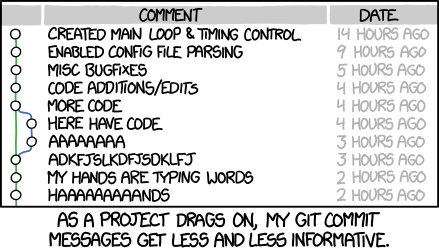
\includegraphics[height=28mm]{GitBadCommits}};
                \node[below = 2mm of L, font=\tiny] {\URL*{https://www.xkcd.com/1296/}{https://www.xkcd.com/1296/}};
            \end{scope}
            \begin{scope}[scope on=<2->]
                \node[right = 1mm of L] (R) {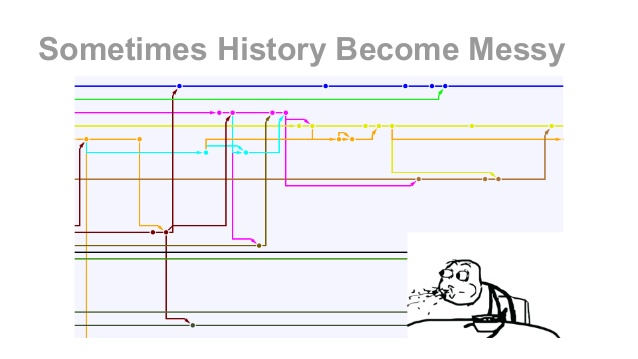
\includegraphics[height=28mm]{GitMessyHistory}};
                \node[below = 2mm of R, font=\tiny]
                    {\URL*{https://image.slidesharecdn.com/gitseries-150826152158-lva1-app6892/95/git-series-episode-3-git-flow-and-githubflow-2-638.jpg?cb=1443100187}{https://image.slidesharecdn.com/[...]}};
                \fill[white] (R.north west) rectangle ($(R.north east)!0.4!(R.east)$);
                \node[font=\footnotesize, anchor=north, fill=white, text=PS] at ($(R.north)-(0,1.5mm)$)
                    {Sometimes history becomes messy};
            \end{scope}
        \end{tikzpicture}
    \end{center}
    \vspace{-3mm}
    \begin{uncoverenv}<3>
        \setlength{\leftmargini}{7mm}
        \begin{itemize}
            \item \alert{Ordered} and \alert{standardized} way to daily work
            \item Easy way to keep big projects history and development tidied up
            \item Sustainable work in team also \alert{for new members}
            \item In larger projects, easy interaction within and between sub-teams
            \item \PP{A way to go for released software}
        \end{itemize}
    \end{uncoverenv}
\end{frame}
%~~~~~~~~~~~~~~~~~~~~~~~~~~~~~~~~~~~~~~~~~~~~%
\begin{frame}[c]{Background}
    \vspace{-3mm}
    \begin{columns}[c]
        \begin{column}{0.5\textwidth}
            \small
            \setlength{\leftmargini}{7mm}
            \begin{itemize}
                \setlength{\itemsep}{0mm}
                \item Central repository (e.g.\ GitHub)
                \item Developers pull/push from/to origin
                \item Sub-team fetches lead to high work efficiency
                \item It might be useful to work together with two or more developers on a big new feature,
                before pushing the work in progress to origin prematurely.
                \item \alert{Never forget \texttt{origin} is public!}
            \end{itemize}
        \end{column}
        \begin{column}{0.45\textwidth}
            \vspace{3mm}
            \centering
            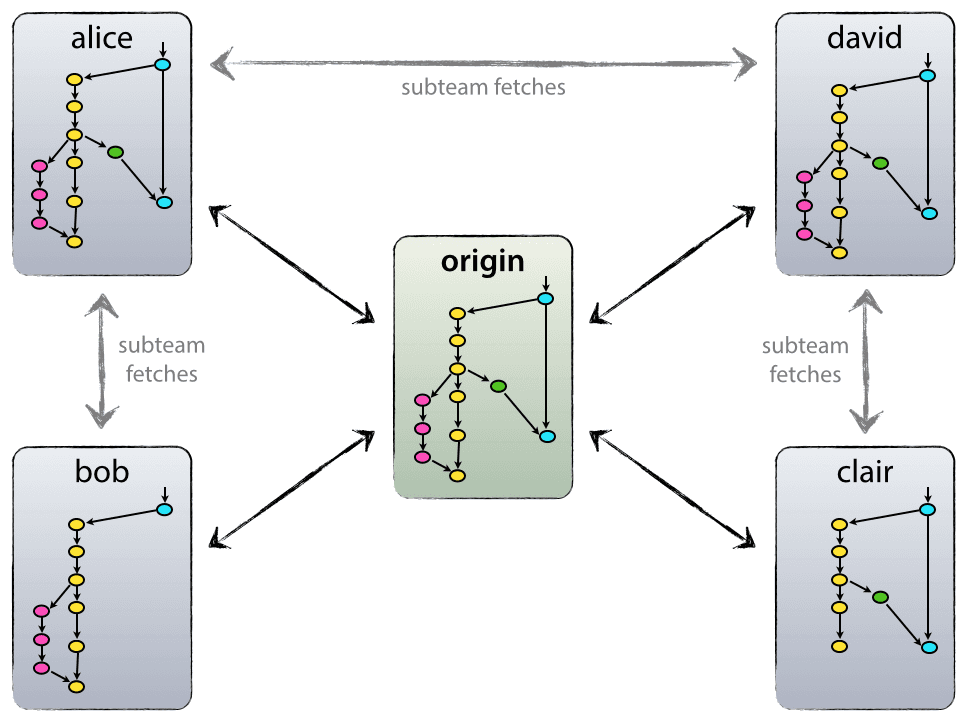
\includegraphics[width=\textwidth]{centr-decentr}
            \begin{block}{}
                \footnotesize\itshape
                Technically, this means nothing more than that, for example, Alice has defined a Git remote,
                named \textnormal{\texttt{bob}}, pointing to Bob's repository, and vice versa.
            \end{block}
        \end{column}
    \end{columns}
\end{frame}
%---------------------------------------------------------------%

%---------------------------------------------------------------%
\subsection{The main branches}
%---------------------------------------------------------------%
\begin{frame}[c]{The main and develop branches}
    \small
    \begin{columns}[b]
        \begin{column}{0.5\textwidth}
            \vspace{-3mm}
            \begin{varblock}{}[0.95\textwidth]{\texttt{origin/\main}}
                The source code of \texttt{HEAD} always reflects a production-ready state
            \end{varblock}
            \vspace{-1mm}
            \begin{varblock}{}[0.95\textwidth]{\texttt{origin/\develop}}
                The source code of \texttt{HEAD} always reflects a state
                with the latest delivered development changes for the next release
            \end{varblock}
            \begin{varblock}{alerted}[0.95\textwidth]{}
                \alert{Each time when changes are merged back into main, this is a new production release by definition}\\
                {\scriptsize $\to$ hooks for enforced policies!}
            \end{varblock}
        \end{column}
        \begin{column}{0.4\textwidth}
            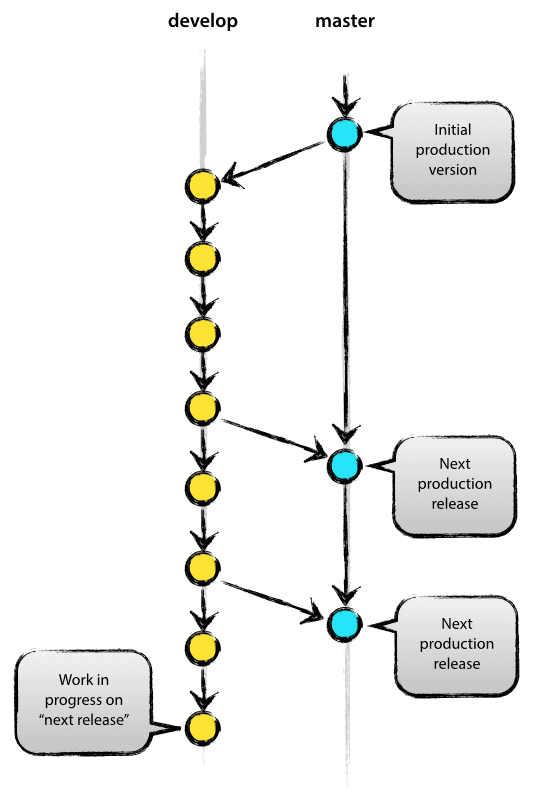
\includegraphics[height=0.77\textheight]{main-branches}
        \end{column}
    \end{columns}
    \FrameRemark{\URL*{https://git-scm.com/book/en/v2/Customizing-Git-Git-Hooks}{Git hooks} are authomatised actions that are triggered by a given git command, i.e.\ git will automatically run a script whenever you run a git command.}
\end{frame}
%---------------------------------------------------------------%

%---------------------------------------------------------------%
\subsection{Feature branches}
%---------------------------------------------------------------%
\begin{frame}[fragile,c]{The feature branches}
    \begin{columns}[c]
        \begin{column}{0.65\textwidth}
            \vspace*{-1cm}
            \begin{overlayarea}{\textwidth}{0.75\textheight}
                \vspace{-3mm}
                \begin{varblock}{}[0.9\textwidth]{Properties}<only@1>
                    \begin{itemize}
                        \item May branch off from:\\
                              \quad{\small\develop}
                        \item Must merge back into:\\
                              \quad{\small\develop}
                        \item Any name except:\\
                              \quad{\small\main,\;\develop}\\[-1mm]
                              \quad{\small\release,\;\hotfix}
                    \end{itemize}
                \end{varblock}
                \vspace{-1mm}
                \begin{varblock}{alerted}[0.9\textwidth]{}<only@1>
                    \small \alert{Feature branches typically exist in developer repository only, not in \texttt{origin}.}
                \end{varblock}
                \vspace{3mm}
                \begin{varblock}{}[1.05\textwidth]{How it looks like:}<only@2>
                    \setlength{\medskipamount}{0pt}
                    \begin{lstlisting}[style=MyBash]
                        $ git switch -c myfeature develop
                        |+Switched to a new branch "myfeature"+|
                        #------------------------------------
                        # Some development, commits, etc.
                        #------------------------------------
                        $ git switch develop
                        |+Switched to branch 'develop'+|
                        $ git pull origin develop
                        |+Already up-to-date.+|
                        $ git merge --no-ff myfeature
                        |+Updating ea1b82a..05e9557
                        (Summary of changes)+|
                        $ git branch -d myfeature
                        |+Deleted branch myfeature (was 05e9557).+|
                        $ git push origin develop
                        |+[...]+|
                    \end{lstlisting}
                \end{varblock}
            \end{overlayarea}
        \end{column}
        \begin{column}{0.3\textwidth}
            \centerline{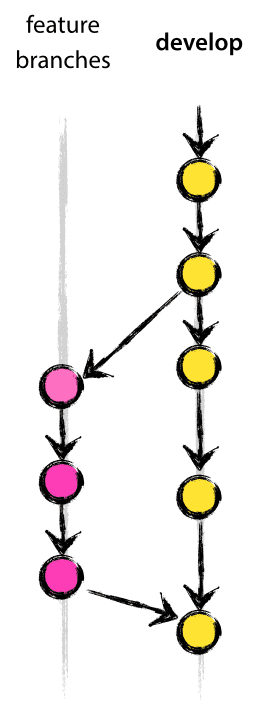
\includegraphics[height=0.75\textheight]{feature}}
        \end{column}
    \end{columns}
\end{frame}
%~~~~~~~~~~~~~~~~~~~~~~~~~~~~~~~~~~~~~~~~~~~~%
\begin{frame}[c]{Why to avoid a fast-forward merge?}
    \begin{tikzpicture}[remember picture, overlay]
        \node[visible on=<1>] at ([yshift=-5mm]current page.center) {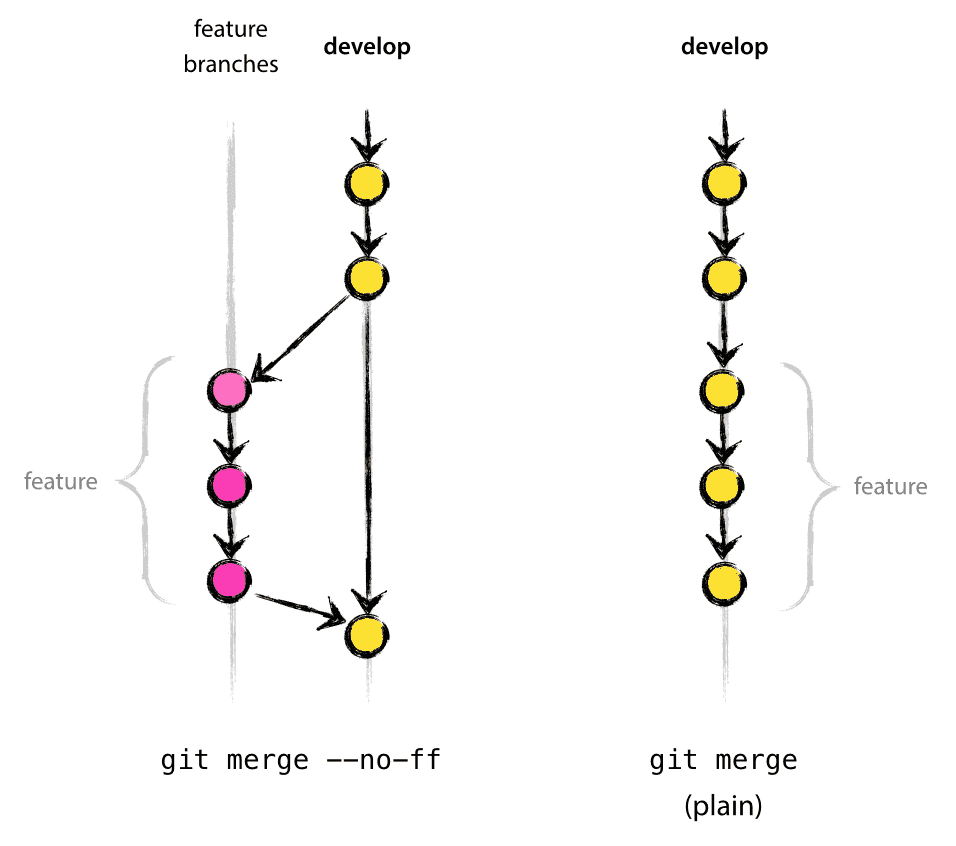
\includegraphics[height=0.65\textheight]{no-ff}};
    \end{tikzpicture}
    \begin{onlyenv}<2>
        \vspace{-8mm}
        \begin{center}
            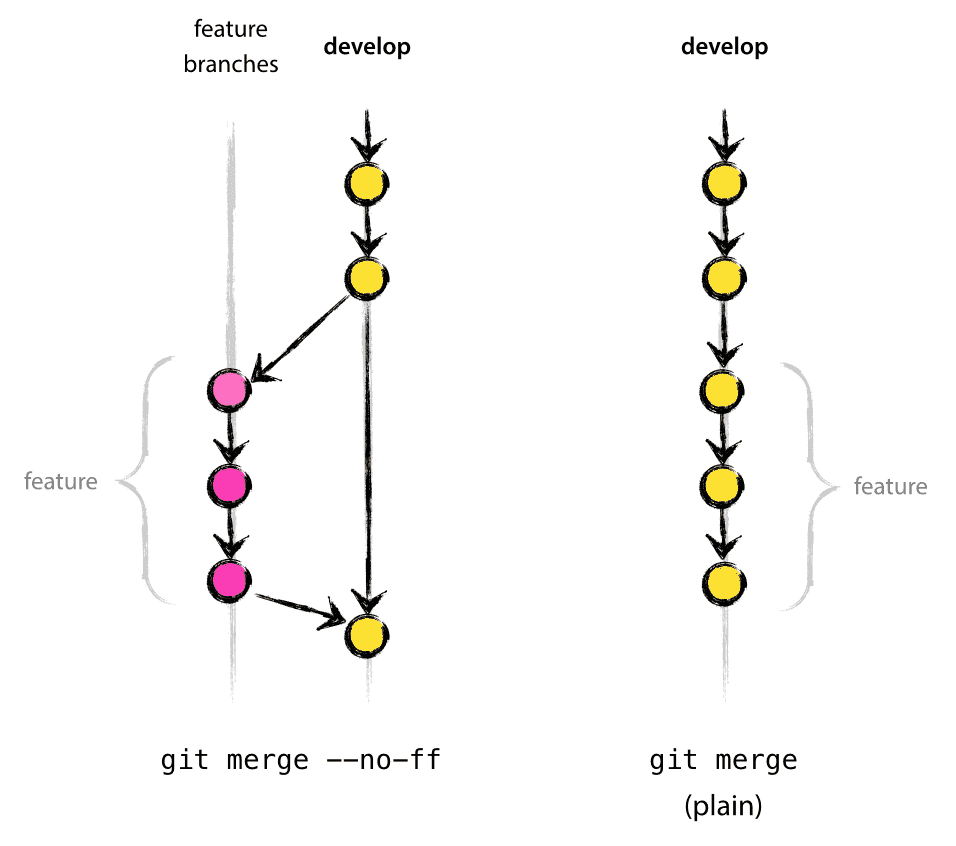
\includegraphics[height=0.35\textheight]{no-ff}
        \end{center}
        \setlength{\leftmargini}{7mm}
        \begin{itemize}
            \setlength{\itemsep}{2mm}
            \item[\checkmark] No information lost about the historical existence of a feature
            \item[\checkmark] Easy to see in history which commits have implemented a feature
            \item[\checkmark] Easy to revert a whole feature (i.e.\ a group of commits)
            \item[\crossmark] It will create (empty) commit objects\\
                              \then the gain is much bigger than the cost!
        \end{itemize}
    \end{onlyenv}
\end{frame}
%---------------------------------------------------------------%

%---------------------------------------------------------------%
\subsection{Release branches}
%---------------------------------------------------------------%
\begin{frame}[fragile,c]{The release branches}
    \begin{tikzpicture}[overlay, remember picture]
        \node[anchor=north east] (yeah) at ([shift={(-8mm,-3mm)}]current page.north east) {
\includegraphics[height=20mm]{SuccessMeme}};
        \path[to] ([shift={(-8mm,-9mm)}]current page.north) edge[out=0, in=180] node[midway, font=\tiny, sloped, above=-3pt]{Make you feel like} (yeah);
    \end{tikzpicture}
    \begin{onlyenv}<2>
        \begin{columns}[c]
            \begin{column}{0.55\textwidth}
                \begin{varblock}{}[\textwidth]{Preperties:}
                    \begin{itemize}
                        \item May branch off from:\\
                        \quad{\small\develop}
                        \item Must merge back into:\\
                        \quad{\small\develop,\;\main}
                        \item Branch naming convention:\\
                        \quad{\small\release}
                    \end{itemize}
                \end{varblock}
            \end{column}
            \begin{column}{0.45\textwidth}
                \vspace{6mm}
                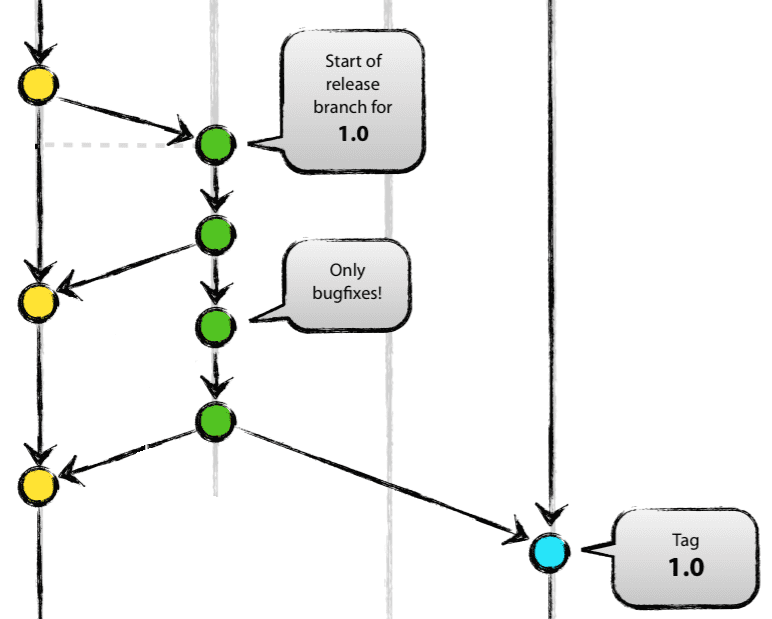
\includegraphics[width=\textwidth]{release}
            \end{column}
        \end{columns}
    \end{onlyenv}
    \begin{onlyenv}<3>
        \begin{minipage}[c]{0.95\textwidth}
            \vspace{14mm}
            \setlength{\leftmargini}{1mm}
            \begin{itemize}
                \setlength{\itemsep}{3mm}
                \item Release branches support preparation of a new production release
                \item Last-minute checks, minor bug fixes and preparing meta-data (version number,
                etc.) should be done on a release branch
                \item By doing all of this work on a release branch, the \textbf{develop}
                branch is cleared to receive features for the following release
                \item \alert{When a new \PQ{release} branch is created, all features that are
                    targeted for this release must be merged into the \PQ{develop} branch}
            \end{itemize}
        \end{minipage}
    \end{onlyenv}
\end{frame}
%~~~~~~~~~~~~~~~~~~~~~~~~~~~~~~~~~~~~~~~~~~~~%
\begin{frame}[fragile,c]{The release branch: How it works}
    \begin{overlayarea}{\textwidth}{0.9\textheight}
        \vspace{-5mm}
        \begin{onlyenv}<1>
            \begin{varblock}{example}{Creation}
                \begin{lstlisting}[style=MyBash]
                    |+Version 1.1.5 is the current production release
                    We are ready for "next release" ->+| |*NOW*| |+we decide v1.2+|
                    $ git switch -c release-1.2 develop
                    |+Switched to a new branch "release-1.2"+|
                    $ ./bump-version.sh 1.2  #Just modify some files
                    |+Files modified successfully, version bumped to 1.2.+|
                    $ git commit -a -m "Bump version number to 1.2"
                    |+[release-1.2 74d9424] Bumped version number to 1.2
                    1 files changed, 1 insertions(+), 1 deletions(-)+|
                \end{lstlisting}
            \end{varblock}
            \begin{varblock}{alerted}[0.8\textwidth]{}
                \alert{Adding new features here is \textbf{strictly prohibited}!}\\
                The idea is to just make sure everything works and is ready to be published!
            \end{varblock}
        \end{onlyenv}
        \begin{onlyenv}<2>
            \begin{varblock}{example}{Creation}
                \begin{lstlisting}[style=MyBash]
                    $ git switch -c release-1.2 develop
                    $ ./bump-version.sh 1.2 #Just modify some files
                    $ git commit -a -m "Bump version number to 1.2"
                \end{lstlisting}
            \end{varblock}
            \vspace{-2mm}
            \begin{varblock}{example}{Finalisation}
                \begin{lstlisting}[style=MyBash]
                    $ git switch main
                    |+Switched to branch 'main'+|
                    $ git merge --no-ff release-1.2
                    |+Merge made by recursive. (Summary of changes)+|
                    $ git tag -a v1.2
                    $ git switch develop
                    |+Switched to branch 'develop'+|
                    $ git merge --no-ff release-1.2  #Maybe conflicts!
                    |+Merge made by recursive. (Summary of changes)+|
                    $ git branch -d release-1.2
                    |+Deleted branch release-1.2 (was ff452fe).+|
                \end{lstlisting}
            \end{varblock}
        \end{onlyenv}
    \end{overlayarea}
\end{frame}
%---------------------------------------------------------------%

%---------------------------------------------------------------%
\subsection{Hotfix branches}
%---------------------------------------------------------------%
\begin{frame}[fragile,c]{The hotfix branch}
    \begin{tikzpicture}[remember picture, overlay, visible on=<2>]
        \node[inner sep=0pt] (yeah) at ([yshift=-8mm]current page.center) {
\includegraphics[height=40mm]{HotfixMeme}};
        \node[below = 2mm of yeah, font=\scriptsize, text=PQ] {\ldots{}and, after all, never forget Murphy's law!};
        \node[above = 4mm of yeah, font=\Large, text=PT] {A hotfix is not something bad!};
        \draw[red, line width=1mm, shorten <= -1mm, shorten >= -1mm] (yeah.south west) -- (yeah.north east);
    \end{tikzpicture}
    \begin{onlyenv}<3>
        \vspace{-9mm}
        \begin{columns}[c]
            \begin{column}{0.55\textwidth}
                \begin{varblock}{}[\textwidth]{Properties:}
                    \begin{itemize}
                        \item May branch off from:\\
                              \quad{\small\main}
                        \item Must merge back into:\\
                              \quad{\small\develop,\;\main}
                        \item Branch naming convention:\\
                              \quad{\small\hotfix}
                    \end{itemize}
                \end{varblock}
                \vspace{-2mm}
                \begin{varblock}{alerted}{Main advantage}
                    \small
                    The essence is that work on the develop branch can continue, while a quick production fix is prepared
                \end{varblock}
            \end{column}
            \begin{column}{0.45\textwidth}
                \vspace{5mm}
                \centerline{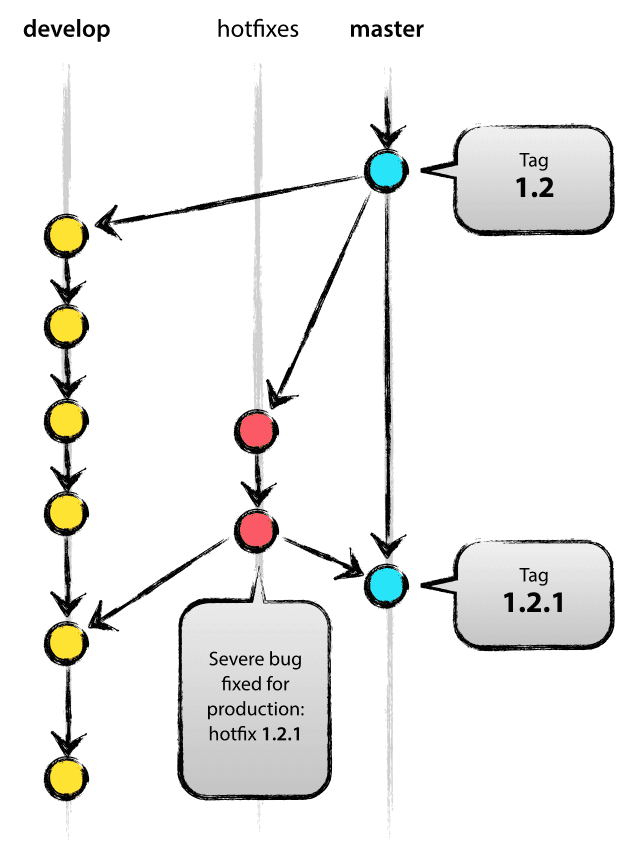
\includegraphics[width=0.9\textwidth]{hotfix}}
            \end{column}
        \end{columns}
    \end{onlyenv}
\end{frame}
%~~~~~~~~~~~~~~~~~~~~~~~~~~~~~~~~~~~~~~~~~~~~%
\begin{frame}[fragile,c]{The hotfix branch: How it works}
    \vspace{-13mm}
    \begin{overlayarea}{\textwidth}{0.8\textheight}
        \begin{onlyenv}<1>
            \begin{varblock}{example}{Creation}
                \begin{lstlisting}[style=MyBash]
                    $ git switch -c hotfix-1.2.1 main
                    |+Switched to a new branch "hotfix-1.2.1"+|
                    $ ./bump-version.sh 1.2.1  #Just modify some files
                    |+Files modified successfully, version bumped to 1.2.1.+|
                    $ git commit -a -m "Bump version number to 1.2.1"
                    |+[hotfix-1.2.1 41e61bb] Bump version number to 1.2.1
                    1 files changed, 1 insertions(+), 1 deletions(-)+|
                    # Some work to fix the situation
                    $ git commit -m "Fix severe production problem"
                    |+[hotfix-1.2.1 abbe5d6] Fix severe production problem
                    5 files changed, 32 insertions(+), 17 deletions(-)+|
                \end{lstlisting}
            \end{varblock}
        \end{onlyenv}
        \begin{onlyenv}<2>
            \begin{varblock}{example}{Creation}
                \begin{lstlisting}[style=MyBash]
                    $ git switch -c hotfix-1.2.1 main
                    $ ./bump-version.sh 1.2.1 #Just modify some files
                    $ git commit -a -m "Bump version number to 1.2.1"
                    # Some work to fix the situation
                    $ git commit -m "Fix severe production problem"
                \end{lstlisting}
            \end{varblock}
            \vspace{-3mm}
            \begin{varblock}{example}{Finalisation}
                \begin{lstlisting}[style=MyBash]
                    $ git switch main
                    |+Switched to branch 'main'+|
                    $ git merge --no-ff hotfix-1.2.1
                    |+Merge made by recursive. (Summary of changes)+|
                    $ git tag -a v1.2.1
                    $ git switch develop
                    |+Switched to branch 'develop'+|
                    $ git merge --no-ff hotfix-1.2.1
                    |+Merge made by recursive. (Summary of changes)+|
                    $ git branch -d hotfix-1.2.1
                    |+Deleted branch hotfix-1.2.1 (was abbe5d6).+|
                \end{lstlisting}
            \end{varblock}
        \end{onlyenv}
    \end{overlayarea}
\end{frame}
%---------------------------------------------------------------%

%---------------------------------------------------------------%
\subsection{Git-flow: an additional tool}
%---------------------------------------------------------------%
\begin{frame}[c]{Summary}
    \begin{tikzpicture}[remember picture, overlay]
        \node[anchor=west] (boss) at ([xshift=10mm]current page.west)
            {
\includegraphics[width=20mm, clip, trim=25mm 0 25mm 0]{LikeABoss}};
        \node[right = 8mm of boss]{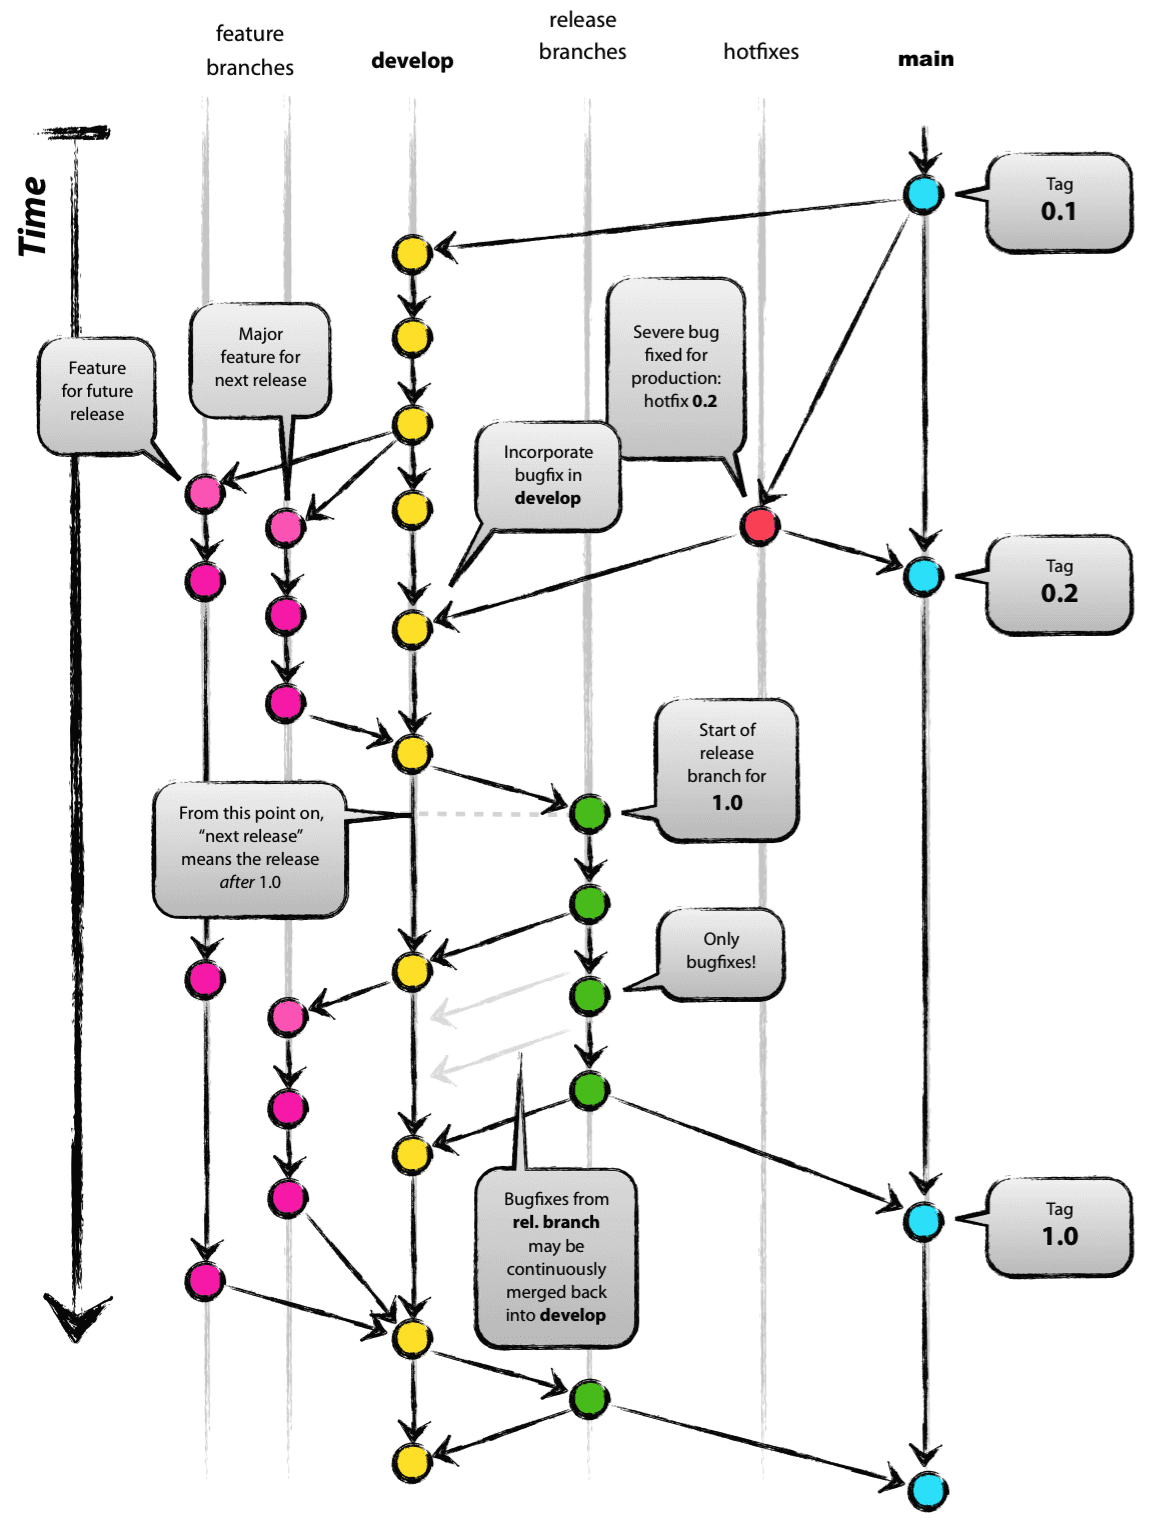
\includegraphics[height=\textheight]{Git-Model}};
    \end{tikzpicture}
\end{frame}
%~~~~~~~~~~~~~~~~~~~~~~~~~~~~~~~~~~~~~~~~~~~~%
\AlertFrame{%
    \begin{tabular}{c}
        
\includegraphics[width=3cm, clip, trim=0 50mm 0 20mm]{ConfusedMeme}\\
        But, wait, everything by hand?!\\[0.55\textheight]
        ~
    \end{tabular}
}
%~~~~~~~~~~~~~~~~~~~~~~~~~~~~~~~~~~~~~~~~~~~~%
\begin{frame}[fragile,c]{Gitflow: How to easily apply what we learnt}
    \vspace{-16mm}
    \begin{overlayarea}{\textwidth}{0.7\textheight}
        \begin{varblock}{example}[0.95\textwidth]{Pick a set of high-level repository operations}
            \PT{\href{https://github.com/nvie/gitflow}{\faGithub\;\textbf{nvie}}}
            \quad or probably better \quad
            \PP{\href{https://github.com/petervanderdoes/gitflow-avh}{\faGithub\;gitflow-avh}}
            \Remark{it has autocompletion}
        \end{varblock}
        \begin{onlyenv}<2>
            \vspace{-3mm}
            \centerline{\scriptsize \hspace{42mm}$\to\;$Standard raw git commands can be used as usual, too}
            \vspace{-6mm}
            \begin{varblock}{example}[0.9\textwidth]{The base syntax}
                \begin{lstlisting}[style=MyBash, aboveskip=2mm]
                    # To initialize a new repository, use:
                    git flow init |+[-d]+|
                    # To list/start/finish auxiliary branches, use:
                    git flow <type>
                    git flow <type> start <name> |+[<base>]+|
                    git flow <type> finish <name>
                    # To push/pull an auxiliary branch to the remote, use:
                    git flow <type> publish <name>
                    git flow <type> pull <remote> <name>
                \end{lstlisting}
                \begin{itemize}
                    \footnotesize\setlength{\itemsep}{0mm}
                    \item[] \bash|<type>|\; can be either \;\texttt{feature}, \;\texttt{release}\; or \;\texttt{hotfix}\\
                    \item[] \bash|<name>|\; is the name of the auxiliary branch\\
                    \item[] \bash{|+<base>+|}\; must be a commit on \;\texttt{develop}\; or \;\texttt{main}
                \end{itemize}
            \end{varblock}
        \end{onlyenv}
        \begin{varblock}{alerted}[0.72\textwidth]{Take-home message}<only@3>
            If you have a released software or plan to have one, Gitflow branching model can help you to bring your product to another level!
        \end{varblock}
        \begin{varblock}{}[\textwidth]{Think about it}<only@3>
            Even if you use a (slightly) different branching model, it might well be that available git extensions still partially fit your use case
        \end{varblock}
    \end{overlayarea}
\end{frame}
%===============================================================%


%===============================================================%
\section{Summary and outlook}
%~~~~~~~~~~~~~~~~~~~~~~~~~~~~~~~~~~~~~~~~~~~~%
\begin{frame}[fragile]{What did we left out in this git trilogy?}
    \begin{tabular}{>{\bfseries\color{PB}}r>{\small}l}
        git mv       & Move or rename a file, a directory, or a symlink \Remark{pretty trivial}\\
        git rm       & Remove files from the working tree and from the index \Remark{pretty trivial}\\
        git restore  & Restore working tree files \Remark{we mentioned it already}\\
        git reset    & Reset current HEAD to the specified state\\
        git blame    & Find out who modified each line in each file\\
        git revert   & Create new commits to undo existing ones\\
        git bisect   & Use binary search to find the commit that introduced a bug\\
        git grep     & Print lines matching a pattern\\
        git [...]    & Few more technical commands
    \end{tabular}
    \begin{varblock}{alert}[\textwidth]{Go for it!}<uncover@2>
        Read your favourite source, you'll be able to understand it alone!
    \end{varblock}
\end{frame}
%~~~~~~~~~~~~~~~~~~~~~~~~~~~~~~~~~~~~~~~~~~~~%
\tikzset{
    opacityOv/.style args={#1on#2}{%
        alt=#2{opacity=#1,text opacity=#1}{}
    }
}
\begin{frame}[plain]
    \PrepareURLsymbol[PT]
    \begin{tikzpicture}[remember picture, overlay]
        \node[anchor=north west, font=\Large, text=PP] at ([shift={(2mm,-2mm)}]current page.north west){Most used Git commands};
        \node[anchor=south] at ([yshift=1mm]current page.south){
            \begin{tikzpicture}
                \only<1>{ %Coordinates shall be set once for all overlays, if not one gets in troubles with counter redefinition!
                    \IfFileExists{./\jobname.pos}{
                        \newcounter{NodeIndex}
                        \immediate\write18{./Sort-TikZ-node-Position.bash} %needs --enable-write18 in compilation
                        %Inspired from https://tex.stackexchange.com/a/48770/128737
                        \pgfplotstableread[header=false]{\jobname.pos}\datatable
                        \pgfplotstableforeachcolumnelement{[index]0}\of\datatable\as\x{
                            \stepcounter{NodeIndex}
                            \pgfplotstablegetelem{\pgfplotstablerow}{[index]1}\of\datatable
                            \coordinate (C\theNodeIndex) at (\x,\pgfplotsretval);
                        }
                    }{
                        \pgfmathsetseed{2}
                        \PlaceSpreadCoordinatesAndStoreThemToFile{0.85\textwidth}{0.78\textheight}{1.25}{26}
                    }
                }
                \begin{scope}[every node/.style={circle, draw, thick, font=\small, inner sep=1mm}]
                    \foreach \s [count=\i from 1] in {config, help}{
                        \node [PB, visible on=<1->, opacityOv=0.3 on <2->] (N\i) at (C\i) {\vphantom{ph}\s};
                    }
                    \foreach \s [count=\i from 3] in {init, clone}{
                        \node [PP, visible on=<2->, opacityOv=0.3 on <3->] (N\i) at (C\i) {\vphantom{ph}\s};
                    }
                    \foreach \s [count=\i from 5] in {add, status, commit, mv, rm, reset}{
                        \node [PS, visible on=<3->, opacityOv=0.3 on <4->] (N\i) at (C\i) {\vphantom{ph}\s};
                    }
                    \foreach \s [count=\i from 11] in {tag, branch, merge, switch, stash}{
                        \node [PT, visible on=<4->, opacityOv=0.3 on <5->] (N\i) at (C\i) {\vphantom{ph}\s};
                    }
                    \foreach \s [count=\i from 16] in {fetch, pull, push, remote}{
                        \node [PQ, visible on=<5->, opacityOv=0.3 on <6->] (N\i) at (C\i) {\vphantom{ph}\s};
                    }
                    \foreach \s [count=\i from 20] in {show, log, diff}{
                        \node [Marine, visible on=<6->, opacityOv=0.3 on <7->] (N\i) at (C\i) {\vphantom{ph}\s};
                    }
                    \foreach \s [count=\i from 23] in {rebase, revert, bisect, blame}{
                        \node [TEXT, visible on=<7->, opacityOv=0.3 on <8->] (N\i) at (C\i) {\vphantom{ph}\s};
                    }
                \end{scope}
                \begin{scope}[every node/.style={font=\footnotesize}]
                    \node[visible on=<1>, above = 4mm of N1, PB] {Setup and Config};
                    \node[visible on=<2>, right = 4mm of N4, PP] {Getting and creating projects};
                    \node[visible on=<3>, above = 4mm of N8, PS] {Basic snapshotting};
                    \node[visible on=<4>, right = 4mm of N14, PT] {Branching and merging};
                    \node[visible on=<5>, right = 4mm of N16, PQ] {Sharing and updating projects};
                    \node[visible on=<6>, right = 4mm of N20, Marine] {Inspection and comparison};
                    \node[visible on=<7>, above = 4mm of N26, TEXT] {Patching and debugging};
                \end{scope}
            \end{tikzpicture}
        };
        \node[visible on=<8->, anchor=north east, font=\small, draw=PT, thick, rounded corners]
        at ([shift={(-3mm,-2mm)}]current page.north east) {\URL*[PT]{https://git-scm.com/docs}{Git Documentation}};
        \begin{scope}[every node/.style={visible on=<9->, opacity=0.85}]
            \node (V) at (current page.center){
\includegraphics[width=0.85\textwidth]{V}};
            \node[anchor=south west] at (V.south west) {
\includegraphics[width=15mm]{Vlogo}};
            \node[anchor=east, text=BGLIGHT] at ([xshift=-4mm]V.center) {
                \begin{tabular}{c}
                    There is\\
                    no certainty,\\
                    only opportunities!\\
                \end{tabular}
            };
        \end{scope}
    \end{tikzpicture}
\end{frame}
%~~~~~~~~~~~~~~~~~~~~~~~~~~~~~~~~~~~~~~~~~~~~%
\begin{frame}{Thanks for listening and remember}
    \begin{varblock}{alert}[\textwidth]{In case of fire:}
        \begin{enumerate}
            \item \bash|git switch -c dfjaskjdsgk|
            \item \bash|git commit -am 'fvfsdavg'|
            \item \bash|git push|
            \item Exit the building
        \end{enumerate}
    \end{varblock}
    \vspace{3mm}
    \begin{tabular}{cc}
        \parbox[c]{3cm}{
\includegraphics[width=3cm]{MemeNotSure}} &
        Not sure whether I need an alias for that...\\
    \end{tabular}
    \vspace{5mm}
    \begin{center}
        \Large \PP{Questions? \; Feedback?}
    \end{center}
    \FrameRemark{In case you are not a fan of memes, sorry for that. I still hope you enjoyed the trilogy!}
\end{frame}
%===============================================================%


\end{document}
